\documentclass{standalone}
\usepackage{tikz}
\usepackage{ctex,siunitx}
\setCJKmainfont{Noto Serif CJK SC}
\usepackage{tkz-euclide}
\usepackage{amsmath}
\usetikzlibrary{patterns, calc}
\usetikzlibrary {decorations.pathmorphing, decorations.pathreplacing, decorations.shapes,}
\begin{document}
\small
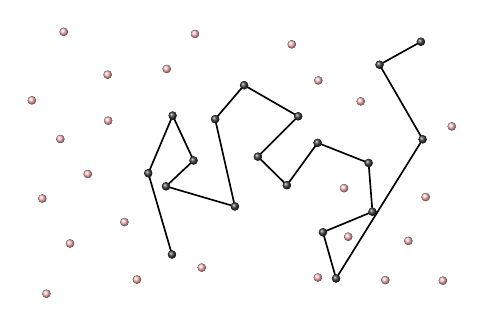
\begin{tikzpicture}[>=latex,scale=1.0]
  \foreach \x/\y in {-2.231/ 1.575,-2.636/ 0.705,-2.274/ 0.214,-2.503/-0.542,-2.151/-1.113,-2.450/-1.751,-1.301/-1.571,-1.460/-0.841,-1.925/-0.231,-1.666/ 0.447,-1.673/ 1.031,-0.923/ 1.104,-0.564/ 1.548, 0.665/ 1.416, 1.003/ 0.958, 1.541/ 0.692, 1.329/-0.410,-0.478/-1.419, 0.997/-1.545, 1.382/-1.027, 1.853/-1.578, 2.584/-1.585, 2.146/-1.080, 2.365/-0.523, 2.697/ 0.374}
  {
    \fill[ball color=pink](\x,\y) circle (1.5pt);
  }
  \draw[semithick](-0.856,-1.253)--(-1.157,-0.221)--(-0.847, 0.511)--(-0.582,-0.059)--(-0.932,-0.387)--(-0.057,-0.643)--(-0.308, 0.466)--( 0.060, 0.897)--( 0.747, 0.502)--( 0.235,-0.010)--( 0.603,-0.373)--( 0.994, 0.165)--( 1.641,-0.091)--( 1.690,-0.710)--( 1.061,-0.970)--( 1.228,-1.558)--( 2.328, 0.210)--( 1.780, 1.157)--( 2.305, 1.449);
  \foreach \x/\y in {-0.856/-1.253,-1.157/-0.221,-0.847/ 0.511,-0.582/-0.059,-0.932/-0.387,-0.057/-0.643,-0.308/ 0.466, 0.060/ 0.897, 0.747/ 0.502, 0.235/-0.010, 0.603/-0.373, 0.994/ 0.165, 1.641/-0.091, 1.690/-0.710, 1.061/-0.970, 1.228/-1.558, 2.328/ 0.210, 1.780/ 1.157, 2.305/ 1.449}
  {
    \fill[ball color=darkgray](\x,\y) circle (1.5pt);
  }
\end{tikzpicture}
\end{document}